%Préambule du document :
\documentclass[12pt, a4paper]{book}
%\usepackage[latin1]{inputenc} 

\usepackage{graphicx}
\usepackage{titling}
\usepackage{amssymb} 
\usepackage{minitoc} % chapter's tocs
\usepackage{fancyhdr} % modify the headers
\usepackage{tabularx} % tables not larger than A4
\usepackage[table]{xcolor} %colours inside the tables
\usepackage{float}
\usepackage{multicol} % multiple columns in some sections
\usepackage[inner=2cm,outer=2cm]{geometry} %A4 margins

\usepackage[labelfont=bf]{caption} % for figure captions in minipages

\pagestyle{fancy}
\fancyhead{}
\fancyfoot{}
\fancyhead[RO,LE]{\thepage}
\fancyhead[LO]{\leftmark}
\fancyhead[RE]{\rightmark}

\setcounter{minitocdepth}{1} %we only want sections in minitoc

\pretitle{%
  \begin{center}
  \LARGE
  
\includegraphics[width=12cm]{Logo_software.png}\\[\bigskipamount]
}
\posttitle{\end{center}}

\title{ISE-MeshTools User's guide\\ISE-MeshTools v1.3}



%\titlepicture[width=13cm]{Logo_software.png}
\author{Renaud LEBRUN}
\date{28th february 2016} 


%Corps du document :
\begin{document}

	\dominitoc

	\maketitle
   ISE-MeshTools is a software designed by Renaud Lebrun, from the University of Montpellier. ISE-MeshTools is a 
system for the processing and editing of series of 3D triangular meshes. The system provides a set of tools for editing, 
positioning, deforming, labeling, measuring and rendering sets of 3D meshes. Features include:
\begin{itemize}
\item Retro-deformation for virtual restoration of fossils/deformed specimens;
\item Point and curve primitives for placing the exact type of landmark points you’re interested in
\item Easy to use 3D interface for positioning and manipulating sets of surfaces and landmark primitives
\item Mesh tagging, labeling and coloring (to allow for the creation of anatomy atlases)
\item Mesh scalar computation and colouring (based upon curvature/thickness etc...)
\end{itemize}


\tableofcontents


		 \chapter{Licence}
    
		\minitoc
		
    \section{ISE-MeshTools}
    ISE-MeshTools is Copyright(C) 2013-2016: Renaud LEBRUN, Cécile PELADAN, Stefan SCHLAGER, Jean DUMONCEL. All rights reserved.
This program is free software; you can redistribute it and/or modify it under the terms of the GNU 
General Public License as published by the Free Software Foundation; either version 2 of the License, 
or any later version.\\\\
This program is distributed in the hope that it will be useful, but WITHOUT ANY WARRANTY; without 
even the implied warranty of MERCHANTABILITY or FITNESS FOR A PARTICULAR PURPOSE. See the 
GNU General Public License for more details.

    \section{VTK}
  ISE-MeshTools’ compiled versions contain binary forms of VTK: Copyright (c) 2000-2006 Kitware Inc. 28 
Corporate Drive, Suite 204, Clifton Park, NY, 12065, USA. All rights reserved. Redistribution and use 
in source and binary forms, with or without modification, are permitted provided that the following 
conditions are met:\\
    Redistributions of source code must retain the above copyright notice, this list of conditions and 
the following disclaimer.\\
    Redistributions in binary form must reproduce the above copyright notice, this list of conditions 
and the following disclaimer in the documentation and/or other materials provided with the distribution.//
    Neither the name of Kitware nor the names of any contributors may be used to endorse or promote products derived from this software without specific prior written permission.\\\\
THIS SOFTWARE IS PROVIDED BY THE COPYRIGHT HOLDERS AND CONTRIBUTORS ``AS IS’’ AND ANY 
EXPRESS OR IMPLIED WARRANTIES, INCLUDING, BUT NOT LIMITED TO, THE IMPLIED WARRANTIES 
OF MERCHANTABILITY AND FITNESS FOR A PARTICULAR PURPOSE ARE DISCLAIMED. IN NO EVENT 
SHALL THE AUTHORS OR CONTRIBUTORS BE LIABLE FOR ANY DIRECT, INDIRECT, INCIDENTAL, SPECIAL, 
EXEMPLARY, OR CONSEQUENTIAL DAMAGES (INCLUDING, BUT NOT LIMITED TO, PROCUREMENT OF 
SUBSTITUTE GOODS OR SERVICES; LOSS OF USE, DATA, OR PROFITS; OR BUSINESS INTERRUPTION) 
HOWEVER CAUSED AND ON ANY THEORY OF LIABILITY, WHETHER IN CONTRACT, STRICT LIABILITY, 
OR TORT (INCLUDING NEGLIGENCE OR OTHERWISE) ARISING IN ANY WAY OUT OF THE USE OF THIS 
SOFTWARE, EVEN IF ADVISED OF THE POSSIBILITY OF SUCH DAMAGE.

		  \chapter{F.A.Q.}
  
    \section{How should I cite ISE-MeshTools in scientific publications ?}
    You may  cite ISE-MeshTools with the following reference :\\
		Lebrun, R. ISE-MeshTools, a 3D interactive fossil reconstruction freeware. 
		12th Annual Meeting of EAVP, Torino, Italy; 06/2014.
    \section{Is ISE-MeshTools a geometric morphometrics software ?}
    No. However, you can digitize 3D landmarks on complex 3D surfaces using ISE-MeshTools, which you 
		can use in other software.
		\section{Can I produce/extract 3D meshes out of CT/MRI data using ISE-MeshTools ?}
		No. To extract 3D meshes CT/MRI data sets, you have to use another software. However, you can edit 
		3D Meshes in various ways using ISE-MeshTools.
		\section{Is there a CTRL-Z functionnality around ?}
		No, there is currently no way to cancel any action. So remember to regularly save your work (especially when tagging surfaces), otherwise precious hours of work can be lost in a second.
     \chapter{Interaction modes}
\minitoc  

 \section{Selection modes}
 \subsection{Normal mode}
Press ``
\includegraphics{images/pixmap/Normal_select_mode.png}" to activate this mode.\\
This is the default selection mode. Selected objects (meshes and landmarks) are drawn ``grey". Unselected ``normal" landmarks are red, while ``target" landmarks are yellow. Unselected meshes can be drawn:
\begin{itemize}
\item Using a uniform colour (default modes)
\item According to tag values at each vertex (tag display mode active 
\includegraphics{images/pixmap/Show_Tag_Window.png})
\item	According to scalar values at each vertex (scalar display mode active 
\includegraphics{images/pixmap/show_color_scale.png} )
\end{itemize}



\subsection{Tag mode}
Press ``
\includegraphics{images/pixmap/Tag_select_mode.png}"to activate this mode
This mode is useful when tagging surfaces (as you can only interact with selected objects). Unselected meshes are drawn ``grey".  Unselected ``normal" landmarks are red, while ``target" landmarks are yellow. Selected landmarks are grey, while selected meshes can be drawn:
\begin{itemize}
\item	Using a uniform colour (default modes)
\item According to tag values at each vertex (tag display mode active 
\includegraphics{images/pixmap/Show_Tag_Window.png})
\item	According to scalar values at each vertex (scalar display mode active 
\includegraphics{images/pixmap/show_color_scale.png} )
\section{Interaction modes}
\end{itemize}

\subsection{Camera mode}
  
\includegraphics{images/pixmap/move.png}``Camera mode" is the default interaction mode, and is active on startup. When active, left and middle mouse button drags result in camera rotation/translation, respectively.
\subsection{Object mode}
   
\includegraphics{images/pixmap/move_mode2.png}When active, left and middle mouse button drags result in object rotation/translation, respectively.
\subsection{Landmark mode}
  
\includegraphics{images/pixmap/Landmarks2.png}When active, only landmarks can be selected/unselected via right mouse button drag/click. This mode is useful when editing/placing landmarks. Left and middle mouse button drags result in camera rotation/translation, respectively.

\section{Landmark setting modes}
Landmarks can be set on surfaces by pressing ``L" + left mouse click. 
Two series of conventional landmarks can be set with ISE-MeshTools: ``normal" and ``target" landmarks. Additionally a third landmark series (``flag" landmarks) can be used to label surface structures. 
\subsection{Normal landmark mode}	
Press ``
\includegraphics{images/pixmap/Landmarks4.png}" to activate this mode (this mode is active by default)
\subsection{Target landmark mode}	

Press ``
\includegraphics{images/pixmap/Landmarks6.png}"  to activate this mode
\subsection{Flag landmark mode}	

Press ``
\includegraphics{images/pixmap/Flag01.png}" to activate this mode

	   \chapter{Keyboard and mouse controls}
\minitoc  

 \section{Keyboard and mouse controls}
\rowcolors{2}{}{gray!25}
\begin{tabularx}{\linewidth}{ | c | X | }
 \hline			
   Ctrl+A & Selects all objects \\ \hline				
   Ctrl+D & Unselects all objects \\ \hline				
   L+ left click & Creates a landmark (either ``normal", ``target" or ``flag" landmark). \\ \hline			
L + right click & If a single landmark is selected, its position is
moved. Nothing happens if no landmark is selected
or if more than one landmark are selected \\ \hline			

Left mouse button drag 
& Camera mode : camera rotation.\newline
 Object mode : object rotation.\newline
Landmark mode : camera rotation. \\ \hline			

Ctrl + left mouse button drag 
& Camera mode : object rotation.\newline
 Object mode : camera rotation.\newline
 Landmark mode : object rotation. \\ \hline	
		
Right mouse button drag & Draws a yellow rectangle. Once right button is
released, all objects (surfaces and landmarks)
falling inside the rectangle get selected/unselected,
depending on their initial selection status \\ \hline	
		
Right mouse button click & All objects (surfaces and landmarks) lying at click
location get selected/unselected, depending on
their initial selection status \\ \hline		
	
Middle mouse button roll (roll wheel) & Zoom / unzoom \\ \hline		
	
Middle mouse button drag 
& Camera mode : camera translation\newline
 Object mode : object translation\newline
 Landmark mode : camera translation \\ \hline	
		
Ctrl + middle mouse button drag 
& Camera mode : object translation\newline
Object mode : camera translation\newline
Landmark mode : object translation \\ \hline			

« Del » & All selected objects are deleted \\ \hline			

T + left click & Tag selected surface with active tag value \\ \hline			
 
T + right click & Tag selected surface with ``0" value \\ \hline			

 \end{tabularx}

\section{Additional controls}
Additional controls are available when using ``lasso cut" or ``lasso tag" (lasso mode should be active):\\
\begin{tabularx}{\linewidth}{ | c | X | }
\hline			
Left click & Adds a segment to polygon (segments are drawn yellow) \\ \hline			

Right click & Connects last segment to first segment. If two segments cross each other, lasso action is canceled. Otherwise, the closed polygon is drawn red.\\ \hline			

Middle click or ``C" + right click. & Once the lasso is closed (lasso polygon drawn red
after a right click), all the vertices falling within the clicked region (outside or inside the polygon) are either:\newline
- given the colour corresponding the the active tag (lasso tag)\newline
- inserted into a new objects (lasso cut).\newline 
See lasso cut and lasso tag sections for further information.\\ \hline	
		
T + left click (``lasso tag" only) & Depending on which tag tool is active, if the
lasso is closed (lasso polygon drawn red after a right click) the vertices are painted either :\newline 
- using the pencil\newline 
- using the magic wand\newline 
- using the flood fill\newline 
Tag propagation is restricted within the area defined by the red polygon.\\ \hline		
	
\end{tabularx}


		\chapter{Camera and object GUI main controls}
\minitoc  

 \section{Camera controls}
\subsection{Camera rotation centre}
By default, the camera rotates around the origin of the coordinate system (x=0, y=0, z=0), but by pressing ``
\includegraphics[scale=0.7]{images/pixmap/Move_cam.png}", the camera will revolve around the centre of mass of all opened objects. The latter option is useful when the centre of mass of an object (or of several ones) is far from the origin of the coordinate system. The grid is drawn using different colors depending on the camera rotation centre (see Fig. \ref{grid_color}). The camera centre can also be set at the location of one of the first 10 ``normal" landmarks (see section \ref{camera_centre_at}).

\begin{figure}
  \centering
  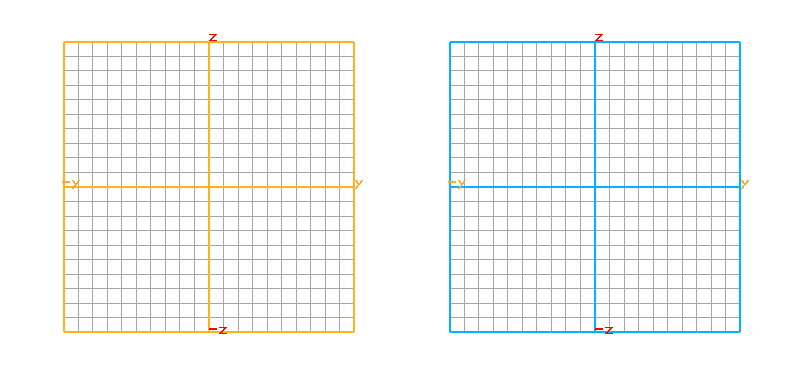
\includegraphics[scale=0.4]{images/GUI/Camera_rotation_centre.png} 
	\caption{Grid display coulour. Left: when the camera revolves around the origin of the coordinate system (x=0, y=0, z=0), the grid is displayed in orange. Right: when the camera revolves around the centre of mass of all opened objects, the grid has a blue layout.}
\label{grid_color}
 
\end{figure}

\subsection{Zoom}
There are three ways to modify the ``zoom" in ISE-MeshTools :


\begin{minipage}{0.7\textwidth}
\begin{itemize}
\item You may use the zoom roller laying in the lower part of the right panel of the main window.
\item	You may open the camera options window (viewing opt. $\rightarrow$  Camera $\rightarrow$ Camera options) and modify manually the ``Zoom" control.
\item	You may set manually the display scale (viewing opt $\rightarrow$ Camera $\rightarrow$ Set 100 pixels in mm)
\item	You may use the middle click mouse roll button (roll the wheel).
\end{itemize}
\end{minipage}    
\begin{minipage}{0.25\textwidth}\centering
  
\includegraphics[scale=0.5]{images/Icons/zoom_01.png}
 \captionof{figure}{Zoom Roll}
 \end{minipage}    


When the option ``Adapt field of view depth" is active in the Rendering options window (Viewing opt.$\rightarrow$General rendering options $\rightarrow$ Depth of field of view panel), changing the zoom value will also modify the depth of the field of view (camera.far value) and the position of the clipping plane (camera.tz value). When the option ``Keep current field of view depth" is active, changing the zoom will not affect the camera.far and camera.tz values.

\subsection{Camera rotation around ``z" viewing axis}

\begin{minipage}{0.7\textwidth}
To do so, you may use the slider lying in the upper part of the right panel of the main window.
\end{minipage}    
\begin{minipage}{0.25\textwidth}\centering
  
\includegraphics[scale=0.5]{images/Icons/Rotation_z.png}
 \captionof{figure}{Camera ``z" rotation slider}
 \end{minipage}    



\subsection{Clipping plane}

\begin{minipage}{0.7\textwidth}
In some cases, you may need to displace the viewing clipping plane. To do so, use
the slider lying centrally in the right panel of the main window.\\
You can also modify the clipping plane manually by editing the ``Tz" control in
the camera options window (viewing opt. $\rightarrow$ Camera $\rightarrow$ Camera options).
The buttons 
\includegraphics[scale=0.7]{images/Icons/clipping_plane3.png} and 
\includegraphics[scale=0.7]{images/Icons/clipping_plane2.png} which lie just underneath the clipping plane slider (and
also in the camera option window) also permit to adjust / readjust the position of
the clipping plane at predefined positions :
\begin{itemize}
\item  
\includegraphics[scale=0.7]{images/Icons/clipping_plane3.png}: the clipping plane is placed at z = 0 (all objects having a z coordinate along
z viewing axis smaller than 0 are hidden).
\item	
\includegraphics[scale=0.7]{images/Icons/clipping_plane2.png} : the clipping plane is replaced at its original value : z= - camera.far / 2. This value permits to
view objects having positive and negative coordinates along z viewing axis.

\end{itemize}
\end{minipage}    
\begin{minipage}{0.25\textwidth}\centering
  
\includegraphics[scale=0.5]{images/Icons/clipping_plane.png}
 \captionof{figure}{Camera clipping plane slider}
 \end{minipage}   




\subsection{Camera orientation}
6 camera positions are predefined :\\

\includegraphics[scale=0.7]{images/pixmap/right2.png} view object from right side \\

\includegraphics[scale=0.7]{images/pixmap/left2.png} view object from left side\\

\includegraphics[scale=0.7]{images/pixmap/right2.png} view object from front side (default camera position)\\

\includegraphics[scale=0.7]{images/pixmap/front2.png} view object from back side\\

\includegraphics[scale=0.7]{images/pixmap/above2.png} view object from above\\

\includegraphics[scale=0.7]{images/pixmap/back2.png} view object from below\\

\subsection{Coordinate system orientation helper}
\begin{minipage}{0.7\textwidth}
Press 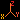
\includegraphics[scale=0.7]{images/pixmap/grid2.png} to show / hide the coordinate system orientation helper lying on the bottom left corner of the main 3D window. By default, the labels are defined
the following way:\\
+z axis : dorsal side\\
-z axis : ventral side\\
+y axis : left side\\
-y axis : right side\\
+x axis : proximal side\\
-x axis : distal side.\\
You may edit these labels depending on your preferences (for instance,
depending on the structure you are working with, you may need to set ``+y" to ``labial", and ``-y" to
``lateral"). To edit orientation labels, click on ``viewing opt. $\rightarrow$ Orientation labels."
\end{minipage}    
\begin{minipage}{0.3\textwidth}\centering
 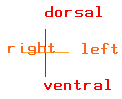
\includegraphics[scale=0.7]{images/GUI/Helper.png}
 \captionof{figure}{Orientation helper}
 \end{minipage}   

\subsection{Grid}
Press 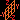
\includegraphics[scale=0.7]{images/pixmap/grid3.png} to show / hide the grid. Default grid size is 1 cm / square. Grid size can be edited manually
(viewing opt. $\rightarrow$ Grid size).
Switching between the 6 camera predefined positions defined above (
\includegraphics[scale=0.7]{images/pixmap/right2.png},
\includegraphics[scale=0.7]{images/pixmap/left2.png},
\includegraphics[scale=0.7]{images/pixmap/right2.png}, 
\includegraphics[scale=0.7]{images/pixmap/front2.png}, 
\includegraphics[scale=0.7]{images/pixmap/above2.png} and 
\includegraphics[scale=0.7]{images/pixmap/back2.png})will
affect the plane in which the grid is drawn.

\subsection{Lightning}
6 lightning orientations are predefined :\\

\includegraphics[scale=0.7]{images/pixmap/s_right_17.png}light from right viewing side\\

\includegraphics[scale=0.7]{images/pixmap/s_left_17.png}light from left viewing side\\

\includegraphics[scale=0.7]{images/pixmap/s_face_17.png}light from front viewing side\\

\includegraphics[scale=0.7]{images/pixmap/s_back_18.png}light from back viewing side\\

\includegraphics[scale=0.7]{images/pixmap/s_dessus_18.png}light from above\\

\includegraphics[scale=0.7]{images/pixmap/s_dessous_18.png}light from below\\

  \section{Object controls controls}
	As seen earlier, selected objects can be translated and rotated using the mouse left and middle buttons
(in landmark and camera selection modes, you also need to maintain ``CTRL" button pressed
while dragging the mouse to achieve rotation and translation of selected objects). Alternatively, you
may also use the following controls to accomplish rotation and translation of selected objects. Rotation
is performed around the global center of mass of all selected objects.

\subsection{Rotation around and translation along ``z" viewing axis}

\begin{minipage}{0.7\textwidth}
These controls are extremely useful, as there is no way to achieve rotation
around « z » viewing axis or translation along ``z" viewing axis using the
mouse. \\
To do so, use the slider and roller lying in the upper part of the left panel of the
main window.

\end{minipage}    
\begin{minipage}{0.25\textwidth}\centering
  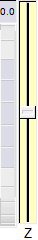
\includegraphics[scale=0.5]{images/Icons/x_rot.png}
 \captionof{figure}{Object ``z" rotation roller and slider}
 \end{minipage}    


\subsection{Rotation around ``x" and translation along ``y" viewing axes}

\begin{minipage}{0.7\textwidth}
To do so, use the slider and roller lying in the lower part of the left panel of the
main window.
\end{minipage}    
\begin{minipage}{0.25\textwidth}\centering
  \includegraphics[scale=0.5]{images/Icons/y_rot.png}
 \captionof{figure}{Object ``x" roller and ``y" slider}
 \end{minipage}   

\subsection{Rotation around ``y" and translation along ``x" viewing axes}


\begin{minipage}{0.5\textwidth}
To do so, use the slider and roller lying in the left part of the bottom panel of the
main window.
\end{minipage}    
\begin{minipage}{0.4\textwidth}\centering
  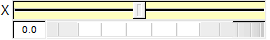
\includegraphics[scale=0.5]{images/Icons/z_rot.png}
 \captionof{figure}{Object ``y" roller and ``z" slider}
 \end{minipage}   


		
\end{document} 
